% State of the Art

\chapter{State of the Art} % Main chapter title

\label{SoA} % For referencing the chapter elsewhere, use \ref{Chapter1} 

\lhead{Chapter 3. \emph{State of the Art}} % This is for the header on each page - perhaps a shortened title

This chapter provides an overview of the topics that supplied the ideas for this thesis. The
following sections examine the previous works which have been done on implementing
Visible Light Communication technology.

%----------------------------------------------------------------------------------------
%	VLC
%----------------------------------------------------------------------------------------

\section{VLC Implementations}

\subsection{Visible Light Communication System Considered}

An indoor visible light communication system using white LEDs under consideration is
shown in \ref{fig:vlc-model}. All the lights in the room are replaced by LEDs. The LEDs
are not only used for illuminating the room but also for an optical wireless
communication system. On-off Keying Return-to-Zero (OOK-RZ) coding is used for
modulating white LEDs. Optical lighting and optical transmission of the white LEDs
have been tested to evaluate the requirements of using VLC for indoor applications. The
effects of the delay problems faced in the high data rate transmission have been studied
and presented in .

\begin{figure}[htbp]
  \centering
    \scalebox{0.6}{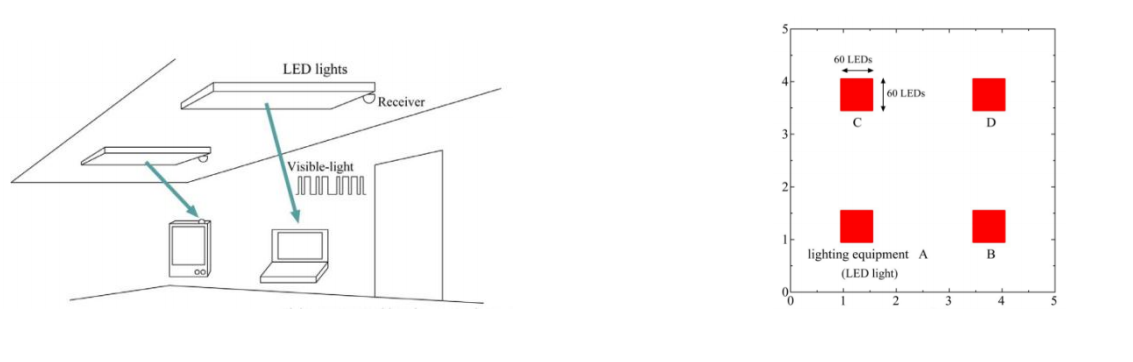
\includegraphics[width=\textwidth]{Pictures/vlc-model-room.png}}
    \rule{35em}{0.5pt}
  \caption[VLC Model Room]{VLC Model Room}
  \label{fig:vlc-model}
\end{figure}

\subsection{Visible Light Road-to-vehicle Communication Using High-Speed Camera}

LEDs are already being used in traffic lights, and they can be used as the communication
medium. Road-to vehicle communication using the LEDs in the traffic signal lights was
proposed.

\begin{figure}[htbp]
  \centering
    \scalebox{0.6}{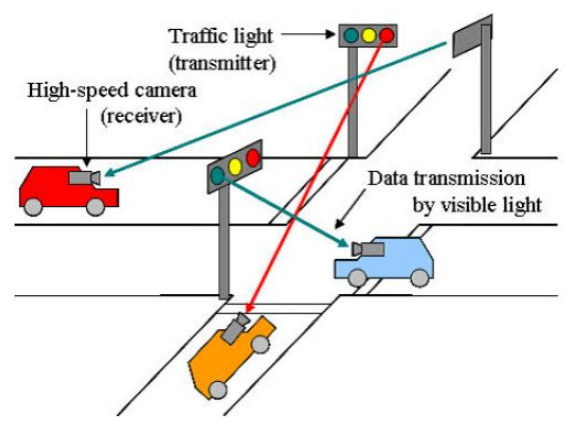
\includegraphics[width=\textwidth]{Pictures/vlc-road.png}}
    \rule{35em}{0.5pt}
  \caption[Road-to-vehicle visible light communication]{Road-to-vehicle visible light communication}
  \label{fig:vlc-road}
\end{figure}

The above \ref{fig:vlc-road} shows the basic usage of LED as a transmitter and CAMERA as a
receiver. In this model, they mounted a camera before the front end of the car. The
camera is used as the information receiver from traffic signal lights. The advantage of
using the camera is that multiple data can be transmitted by the LEDs and received by
High-speed cameras. 


\subsection{Integrated System of White LED Visible-Light Communication and Power-Line Communication}

In [2], optical communication using the existing power-line in a household is proposed as
shown in \ref{fig:vlc-powerline}
The power-line is used for communication between white LEDs and other fixed
networks. The already installed power-lines and outlets behave as data networks and
ports.

\begin{figure}[htbp]
  \centering
    \scalebox{0.6}{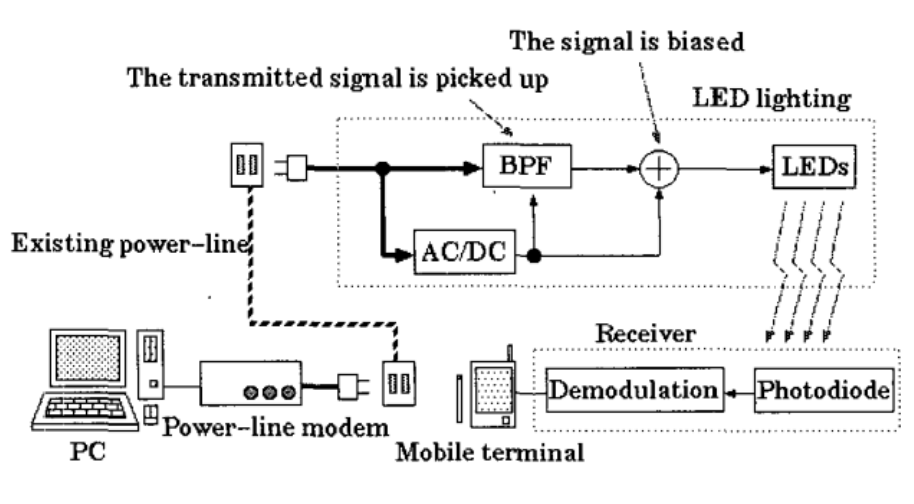
\includegraphics[width=\textwidth]{Pictures/vlc-powerline.png}}
    \rule{35em}{0.5pt}
  \caption[Waveform on power-linel]{Waveform on power-line}
  \label{fig:vlc-powerline}
\end{figure}

As in optical intensity modulation, the transmitted signals are added to the cyclic
waveform of the alternating current (AC). The transmitter signal from the PC is picked
by BPF through the power-line, and biased before sending to the LED lights. The
electrical signal is then converted into an optical signal by LEDs and sends it to the
photodiode, where it converts the captured optical signal to an electrical signal. The
signal is demodulated according to the received level of light and then is passed to the
mobile terminal.

\subsection{Visible Light Communication for Advanced Driver Assistant Systems}

\begin{figure}[htbp]
  \centering
    \scalebox{0.6}{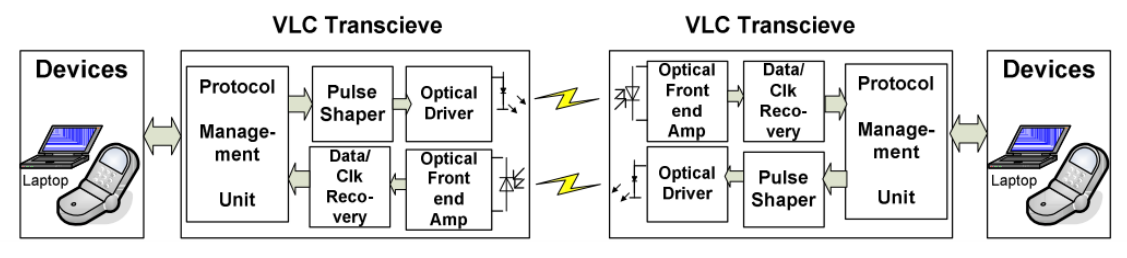
\includegraphics[width=\textwidth]{Pictures/vlc-driver.png}}
    \rule{35em}{0.5pt}
  \caption[General architecture for a full duplex VLC system ]{General architecture for a full duplex VLC system }
  \label{fig:vlc-driver}
\end{figure}

Optical communications for outdoor communication has been discussed and elaborated
upon [4]. Devices such as laptops and mobile phones can be used for transmitting and
receiving information, using transceivers, as shown in \ref{fig:vlc-driver}. Transceiver systems use
both LEDs and photodiodes. Intensity modulation was implemented to reach the most
viable modulation. Various important design parameters were optimized by using
intensive investigation based on gain variation over 100m of transmission range [4]. 

\subsection{Study of Visible Light Communication System Using RGB LED Lights}

Disney research group in Zurih {\citep{disney}} demonstrates a half-duplex VLC LED-to-LED communication with various applications with new generation toys.
First example is a short-range directional communication with
a number of toys, where front and backlights are used to exchange
messages when pointed towards each other. On other application is a LED light bulb in a desk lamp receiving
messages from a mobile device and broadcasts it back to the desk
with higher light intensity and larger coverage. The static lamp acts
as a repeater so that more devices can receive the original messages
and the resulting network connectivity increases.

\subsection{Visible Light Communication using smartphone camera and rolling shutter effect}

Cameras embedded in smartphones can be used as VLC receivers. As a result, common lights and smartphone cameras has the potential to enable a great number
of applications with low cost. In \citep{rolling}, a prototype VLC
system that utilizes undersampled frequency shift ON-OFF keying (UFSOOK) modulation is proposed. The system utilizes rolling shutter cameras as the receiver and takes advantages of its characteristics to improve the receiving performance. An LED is used as the transmitter.
Information is transmitted in the continuous state (ON-OFF) changes of LEDs which are invisible to human eyes. 
The performance evaluation results demonstrate that the communication prototype is robust and can resist common optical interferences and noises within the image.

\subsection{Visible Light Communication using smartphone ambient light sensor}

%----------------------------------------------------------------------------------------
%	SMARTPHONE SOLUTIONS
%----------------------------------------------------------------------------------------

\section{Smartphone solutions}

\subsection{Camera}
\subsection{External peripheral}

%----------------------------------------------------------------------------------------
%	CURRENT RESEARCHES
%----------------------------------------------------------------------------------------

\section{Current researches}